\chapter{Implementation}

In the toy example in Chapter 1, doctors Adam and Barry use different threshold
values on covariate $X$ when making their treatment recommendations. Such
threshold value is referred to a {\it cut} in the implementation. For each
covariate $X$ and a particular cut value $c$, there are two treatment
recommendations, 
\begin{description}
\item[Treatment 1] Give treatment 1 if $X < c$ and treatment 0 otherwise.
\item[Treatment 2] Give treatment 1 if $X \geq c$ and treatment 0 otherwise. 
\end{description}
It is easy to show that $I_{X < c} = I_{A = (X < c)}$ and
$I_{X \geq c} = I_{A = (X \geq c)}$ In the implementation, the bitmask $I_{X<c}$
for each cut is saved.  The  search can then be implemented as follows

\begin{verbatim}
// Depth one 
double v[2] = {0.0}; 
for (size_t i = 0; i < N; ++i) {
  v[0] += y[i] * (a[i] == m[i]);       // X < c
  v[1] += y[i] * (a[i] == 1 - m[i]);   // X >= c
}

// Depth two 
double v[4] = {0.0}; 
for (size_t i = 0; i < N; ++i) {
  // X1 < c1 and X2 < c2
  v[0] += y[i] * (a[i] == m1[i]) * (a[i] == m2[i]); 
  
  // X1 < c1 and X2 >= c2
  v[1] += y[i] * (a[i] == m1[i]) * (a[i] == 1 - m2[i]);

  // X1 >= c1 and X2 < c2
  v[2] += y[i] * (a[i] == 1 - m1[i]) * (a[i] == m2[i]);

  // X1 >= c1 and X2 >= c2 
  v[3] += y[i] * (a[i] == 1 - m1[i]) * (a[i] == 1 - m2[i]);
}
\end{verbatim}

As the depth of search increases, the above implementation becomes
more cumbersome. However, if the package is to be deployed on GPUs,
the above implementation can be revised to utilize vectorization.
Currently, the package is intended to run on multicore computers, and the
computation is organized differently which we explain next.

\begin{figure}[h]
  \centering
  \caption{Demonstration of depth one search}
  \label{fig:depth1}
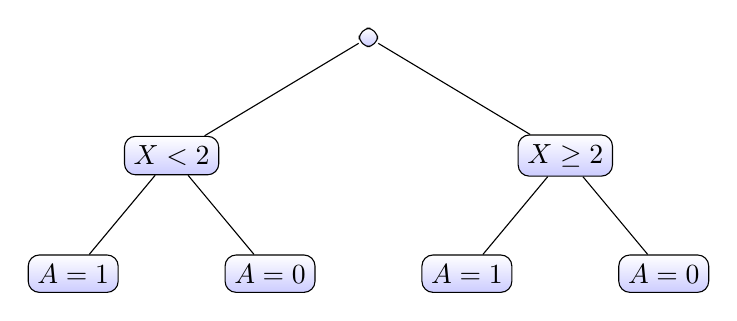
\begin{tikzpicture}[
  level/.style={sibling distance = 5cm/#1,
    level distance = 1.5cm},
  every node/.style = {shape=rectangle, rounded corners,
    draw, align=center,
    top color=white, bottom color=blue!20}
  ]
  \node {} % Root
  % left child
  child { node {$X<2$}
    child { node {$A=1$} }
    child { node {$A=0$} }
  }
  % right child
  child { node {$X \geq 2$}
    child { node {$A=1$} }
    child { node {$A=0$} }
  };
\end{tikzpicture}
\end{figure}

Consider the depth one case shown in Figure~\ref{fig:depth1}. Recall that the
bitmask of $X < 2$ is stored. For each sample $i$ being processed, there are
four combinations depending on the value of $A$ and the bitmask $X(i) < c$. This
means, the corresponding $Y(i)$ can be sorted into four buckets. For instance,
the far left bucket corresponds to $X(i) < c$ and $A=1$ and can therefore be
indexed as bucket 3 ($(11)_2$). The far right bucket can be indexed as bucket 0 (
$(00)_2$). Let $T_0$ be
\[
T_0 = \sum_{i, A(i) = 0} Y(i)
\]
and $B_i$, $i=0,1,2,3$ denote the value accumulated in each bucket.
Notice that
\[B_3 - B_2 + T_0 
=  \{A = 1 \cap X < 2\} - \{A = 0 \cap X < 2\} + \{A = 0\}
= \{A = 1 \cap X < 2\} + \{A = 0 \cap X \geq 2\}
\]
%
If $X(i) < 2$, the recommendation is treatment 1, matching $A(i)$.
If $X(i)\geq 2$, the recommendation is treatment 0, matching $A(i)$. In other
words, the quantity $B_3 - B_2 + T_0$ gives the result for treatment $X < c$.
Similarly, one can verify that $B_1 - B_0 + T_0$ gives the result for
treatment $X \geq c$. 
